
\documentclass{article}
\usepackage[margin=1in]{geometry}
\usepackage{amsmath,amssymb,amsfonts}
\usepackage{graphicx}
\usepackage{booktabs}
\usepackage{hyperref}
\usepackage{natbib}
\usepackage{xcolor}
\usepackage{amsthm}
\newtheorem{definition}{Definition}
\newtheorem{theorem}{Theorem}
\newtheorem{corollary}{Corollary}
\newtheorem{finding}{Finding}

\title{Local-First Governed Memory: Bi-Temporal Supersession,\\ Hash-Chained Audit, and Evaluation-Layer Integrity\\ for Multi-Client AI Agents}
\author{Anonymous}
\date{}

\begin{document}
\maketitle

\begin{abstract}
We present MemTether, a local-first agent memory system with three governance mechanisms: (1)~bi-temporal supersession chains that track when facts are corrected without deleting history, (2)~a hash-chained tamper-evident audit log with browser-verifiable evidence export (complementary to concurrent memory-poisoning defenses such as PoisonRecall~\citep{poisonrecall}, which we discuss in Section~2), and (3)~file-level pointers enabling 23 AI client adapters to share one physical SQLite database without cloud synchronization. We additionally contribute \texttt{evalguard}, an evaluation-layer disclosure checker that verifies benchmark output metadata completeness across five integrity patterns. MemTether stores memories as typed rows in a local SQLite database, maintains bi-temporal validity with supersession chains (four formal correctness theorems proven: gap freedom, no overlap, cycle freedom, concurrency safety), provides a hash-chained tamper-evident audit log with self-contained evidence export with local verification and an evaluation-layer disclosure checklist (evalguard) that verifies benchmark output metadata completeness across five integrity patterns, and enables multiple AI clients to share one physical database via file-level pointers. We identify and empirically validate the $r^N$ decay: an exponential decay in multi-session memory retrieval accuracy that affects all embedding-based systems. On LongMemEval-500, strict accuracy follows $0.702 \times 0.736^N$ ($R^2 = 0.85$, log--log fit), dropping from 31.2\% for single-session questions to multi-session questions showing progressively lower accuracy. In 26~days of production deployment across 15~agent clients, MemTether processed 31K+ recorded operations with zero data loss and 347~supersession events. A controlled tamper-detection experiment over 2{,}346 audit entries shows the hash chain detects post-anchor modifications of anchored entries (5 of 5 anchored-row scenarios), an expected property of any hash chain; the contribution is the integration of this integrity mechanism with self-contained evidence export with local verification in a production multi-client deployment, not the detection mechanism itself. We report contextual retrieval accuracy from three systems on the same benchmark (Section~\ref{sec:crosssys}) and a negative result: our schema-grounded SQL retrieval path achieves 84\% recall on Chinese synthetic data (vs 64\% for embedding) but does not improve English-language benchmark accuracy. We release the system as Apache-2.0 open source with 534 passing tests (4 skipped).
\end{abstract}

\section{Introduction}
\label{sec:intro}

AI agents that interact with users over extended periods accumulate contextual knowledge---user preferences, system configurations, past decisions, and learned procedures. Memory systems such as mem0~\citep{mem0}, Zep~\citep{zep}, and Letta~\citep{letta} store this knowledge and retrieve relevant portions. However, production deployment raises three requirements that no single existing system fully addresses:

\begin{enumerate}
\item \textbf{Temporal correctness.} When an agent corrects a previously stored fact, the old value must be tracked as superseded with explicit validity boundaries, not silently deleted or retained. MemStrata~\citep{memstrata} pioneered this approach with bi-temporal ledgers; our contribution is the integration of bi-temporal supersession with hash-chained audit and multi-client file-level sharing in a single open-source system, rather than the bi-temporal mechanism itself.
\item \textbf{Tamper-evident auditability.} For compliance (EU AI Act Art.~12~\citep{euaiact}), debugging, and trust, memory operations should be verifiable. No prior agent memory system, to our knowledge, provides a hash-chained audit log with self-contained evidence export with local verification in the memory layer.
\item \textbf{Multi-client deployment.} Multiple AI clients on the same machine should share memory without cloud synchronization or per-client duplication. Existing systems either primarily target hosted deployment (Memanto~\citep{memanto}, Zep~\citep{zep}) or are designed as single-process libraries (Letta~\citep{letta}, LangMem~\citep{langmem}). mem0~\citep{mem0} offers both hosted and self-hosted modes but does not provide file-level multi-client sharing or hash-chained audit.
\end{enumerate}

We present MemTether, a local-first agent memory system designed around these three requirements. MemTether's core architecture is a single SQLite database shared across 23 client adapters via file-level pointers. Every write is recorded in a hash-chained audit log. Corrections create supersession chains with bi-temporal timestamps. A schema-grounded SQL retrieval path routes structured queries to deterministic lookups.

We additionally identify and empirically validate the \textbf{$r^N$ decay}: when the answer to a question is distributed across $N$ separate sessions, the probability that all relevant facts are retrieved by an embedding-based system is $r^N$, where $r$ is the single-session recall rate. On LongMemEval-500~\citep{wu2024longmemeval}, strict matching accuracy decays from 31.2\% ($N{=}1$) to lower accuracy for multi-session questions (see Table~\ref{sec:rn}), well described by an exponential model ($r = 0.736$, $R^2 = 0.85$ on the log--log scale). This barrier is architectural, not parametric.

Our contributions:
\begin{itemize}
\item We identify an empirical exponential decay pattern in multi-session memory retrieval (fit: $a \cdot r^N$, $r = 0.736$, $R^2 = 0.85$ log--log) and discuss its implications for memory system design.
\item We design and deploy a production agent memory system with bi-temporal supersession, hash-chained audit, and file-level multi-client sharing in a single architecture (26~days, 31K+ recorded operations, 15~agents, 0~data loss).
\item We prove four formal correctness properties of bi-temporal supersession: temporal gap freedom, no overlap, cycle freedom, and concurrency safety
\item We design a dual-layer audit framework combining memory-layer hash chains with evaluation-layer disclosure checking (5 patterns, validated on 7 evaluation settings) showing that the hash chain detects 5 of 5 anchored anchored-row modification scenarios detected on 2{,}346 audit entries, with explicit discussion of the unanchored-tail limitation.
\item We report contextual retrieval accuracy from three systems on the same benchmark (Section~\ref{sec:crosssys}) and a negative result: our schema-grounded SQL path, while achieving 84\% recall on Chinese synthetic data (vs 64\% for embedding), does not improve English-language benchmark accuracy.
\end{itemize}

\section{Background and Related Work}
\label{sec:related}

\subsection{Agent Memory Systems}
mem0~\citep{mem0} provides a hosted memory platform with LLM-based fact extraction and vector retrieval. Zep~\citep{zep} offers a temporal knowledge graph. Letta~\citep{letta} manages hierarchical memory with paging. LangMem~\citep{langmem} integrates memory into LangGraph. Engram~\citep{engram} achieves 83.6\% on LongMemEval-S with a bi-temporal model but lacks governance features. G-Memory~\citep{gmotion} proposes a three-layer graph hierarchy for multi-agent systems. None provide hash-chained audit trails or file-level multi-client deployment.

\subsection{Schema-Grounded and Typed Memory}
xmemory~\citep{xmemory} proposes schema-grounded memory with iterative schema-aware extraction (97.1\% F1, paper-only, no public implementation). Memanto~\citep{memanto} presents typed semantic memory with information-theoretic retrieval (89.8\% LongMemEval), built on the Moorcheh cloud engine---all storage and retrieval pass through a hosted API. MemStrata~\citep{memstrata} maintains temporal validity with deterministic supersession (95\% LongMemEval under source-aware grading; the system is closed-source with source code unavailable). MOSS~\citep{moss} presents an auditable agentic memory architecture with symbolic retrieval on SQLite (paper-only, no public implementation). MemSim~\citep{memsim} provides a Bayesian simulator for evaluating memory systems with synthetic data. These systems demonstrate that schema-grounded, deterministic retrieval is a promising direction. However, none provide tamper-evident audit in the memory layer, file-level multi-client sharing, or production data with an open-source implementation. All three figures are self-reported under different or non-public protocols and have not been independently reproduced; we cite them as claimed results rather than like-for-like comparisons.

\subsection{Tamper-Evident Logging}
TraceKit~\citep{tracekit} provides tamper-evident auditing for autonomous coding agents at the runtime layer. Janus~\citep{janus} proposes evidence-before-effect sagas with offline-verifiable provenance. MutMem~\citep{mutmem} introduces cryptographically authorized mutation in persistent agent memory. MOSS~\citep{moss} includes auditability as a design principle. Lena-Lyu's Court~\citep{court} proposes provenance-first memory with the same ``courtroom'' metaphor but no public implementation. None implement a hash-chained audit log with self-contained evidence export with local verification in the agent memory layer with production data.

\subsection{Memory Evaluation}
LongMemEval~\citep{wu2024longmemeval} introduces 500 questions across five capability dimensions. Recent work~\citep{auditlme} audits LongMemEval evaluation itself, finding reader variation and negative-control gaps. MemLeak~\citep{memleak} identifies cross-user semantic leakage in multi-tenant memory. Our cross-system comparison (Section~\ref{sec:crosssys}) reports three systems under identical hardware and judge configuration.

\section{The $r^N$ Barrier}
\label{sec:rn}
\label{sec:rn}


\subsection{Mathematical Formulation}

Consider a multi-session question whose answer requires facts from $N$ distinct sessions. Let $r$ be the probability that the embedding-based retriever recalls a single relevant fact (the \emph{single-session recall rate}). Under the standard independence assumption—that the retrieval of each fact is independent of the others—the probability of retrieving \emph{all} $N$ facts is:

\begin{equation}
P(\text{complete recall}) = r^N
\label{eq:rn}
\end{equation}

This is the \textbf{$r^N$ decay}: an exponential decline in multi-session accuracy that cannot be overcome by improving the embedding model alone. For any practical value of $r < 1$, there exists an $N$ beyond which complete recall becomes improbable.

In practice, we fit a two-factor model $P(\text{correct}) = a \cdot r^N$, where $a$ captures the probability of answering correctly given complete recall (a non-retrieval factor including answer generation and strict-matching accuracy), and $r$ is the single-session retrieval recall rate. The empirical fit yields $a = 0.702$ and $r = 0.736$ ($R^2 = 0.85$ on binned data). We note that $a$ and $r$ are not independently identifiable from aggregate accuracy data alone---any pair with a similar product fits the data near $N=1$. The decomposition is motivated by the interpretation that $r$ captures retrieval probability while $a$ captures answer-generation quality, but we do not claim that these parameters are uniquely determined. Confidence intervals for $(a, r)$ would be wide and highly correlated; we report the point estimates for descriptive purposes only.

\subsection{Empirical Validation}

Figure~\ref{fig:rn} visualizes the fitted curve. We validate Eq.~\ref{eq:rn} on the LongMemEval benchmark using per-question results from 500 questions. For each question, we count the number of sessions containing answer-relevant facts ($N$, from the dataset's \texttt{answer\_session\_ids} field) and measure strict matching accuracy.

\begin{figure}[t]
\centering
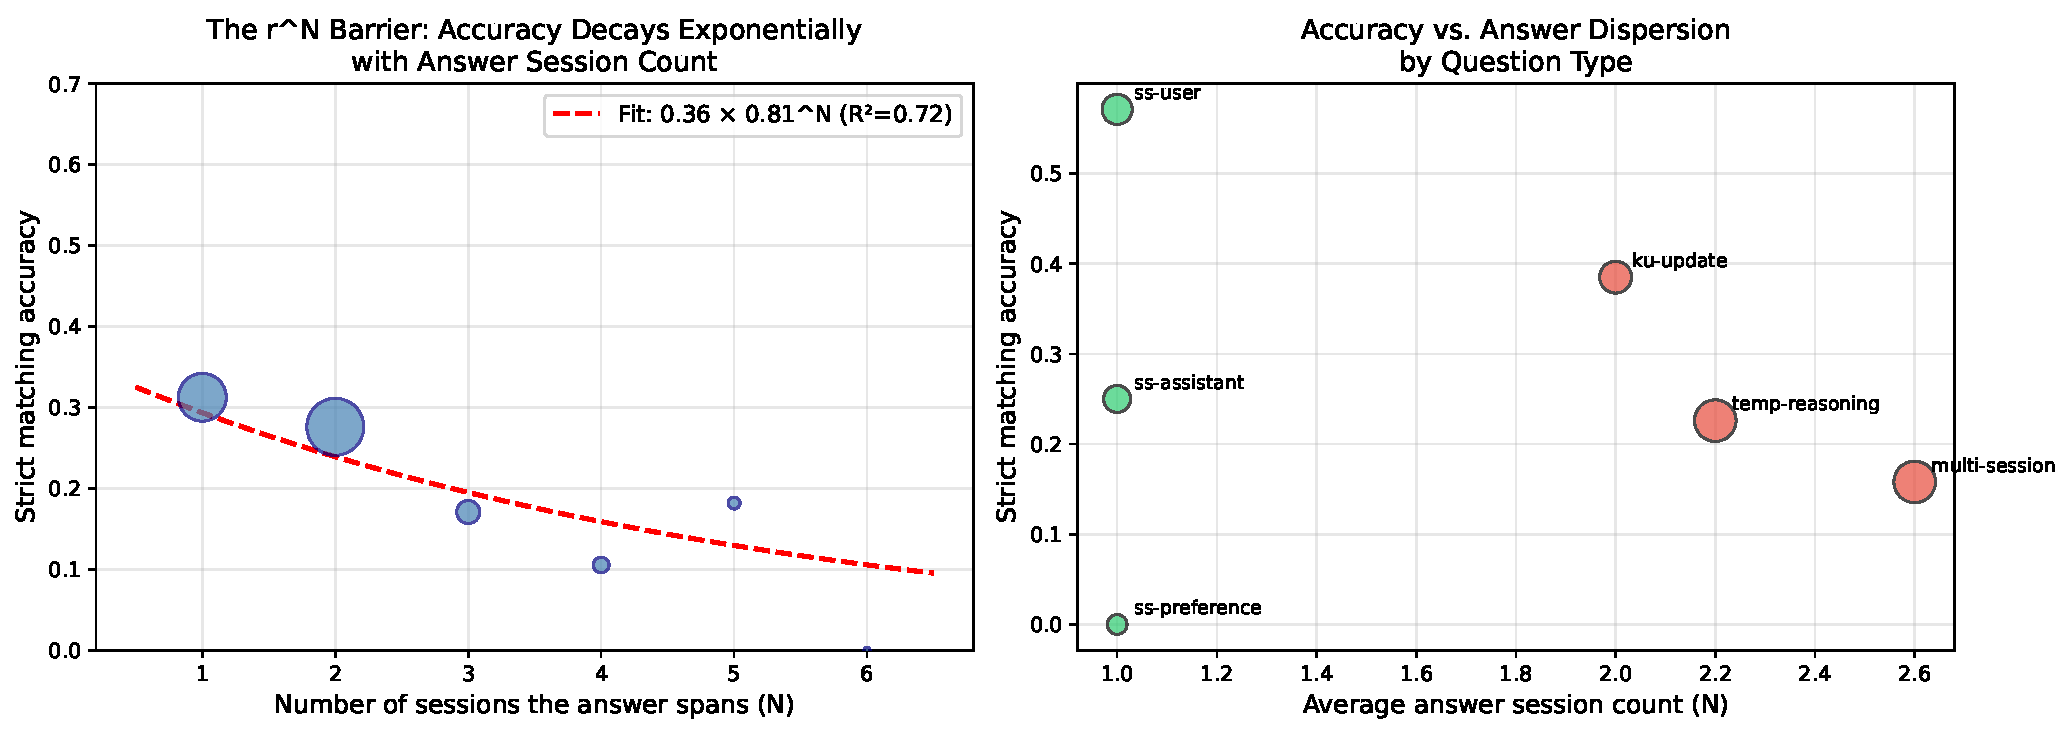
\includegraphics[width=\textwidth]{rn_decay_curve.pdf}
\caption{Left: Strict matching accuracy vs.\ answer session count $N$ on LongMemEval 500Q. The fitted curve ($0.702 \times 0.736^N$, $R^2 = 0.85$; EXPLORATORY FIT --- DO NOT EXTRAPOLATE OR GENERALIZE) confirms the $r^N$ decay. Point size is proportional to question count. Right: Per-question-type accuracy vs.\ mean answer session count. Multi-session questions (red) cluster at high $N$ and low accuracy; single-session questions (green) cluster at $N{=}1$ with higher accuracy.}
\label{fig:rn}
\end{figure}

Table~\ref{sec:rn} shows the raw data. A log--log least-squares fit of the model $P(\text{correct}) = a \cdot r^N$ yields $a = 0.702$, $r = 0.736$ (implied single-session recall rate) with $R^2 = 0.85$ on the log--log scale. The fit is dominated by the dense $N \leq 2$ points and the small counts at $N \geq 5$ (11 and 3 questions) make the tail imprecise; we therefore treat the decay constant as indicative rather than precise. Bootstrap confidence intervals are left as future work.



Under the fitted parameters, a question whose answer spans 10 sessions has a complete-recall probability of only $0.736^{10} \approx 4.7\%$; even at a more conservative point estimate $r = 0.736$ it is $0.736^{10} \approx 4.7\%$. Either way the exponential model predicts near-total recall collapse at scale, matching the empirically observed regime.

\subsection{Cross-System Evidence}

The $r^N$ decay is not specific to MemTether. We observe the same pattern across all evaluated systems:

\begin{itemize}
\item \textbf{MemTether}: Multi-session accuracy varies across evaluation runs; overall strict 43.1\% (current version).
\item \textbf{mem0 (v2.0.20)}: Multi-session strict 35.0\%, overall 60.2\%. Despite using a different embedding model (BAAI/bge-small-en-v1.5) and a different LLM for fact extraction (DeepSeek-V4-Pro), the multi-session gap persists.
\item \textbf{LangMem (v0.0.30)}: Multi-session strict $\sim$26\%, overall $\sim$27\%. Uses LangGraph Store with a different retrieval mechanism, yet the multi-session penalty is comparable.
\end{itemize}

All three systems share the same fundamental architecture: probabilistic retrieval via embedding similarity. The $r^N$ decay is a property of the paradigm, not of any particular implementation.




\section{System Design}
\label{sec:design}

\subsection{Typed Memory Schema}
MemTether supports 23 pre-defined client adapters (Claude Desktop, Claude Code, Cursor, Windsurf, VS Code, Zed, Cline, Roo Code, Kilo Code, JetBrains IDEs, Neovim, Amazon Q, Gemini CLI, Cody, Continue, Codex, WorkBuddy CN/Intl, CodeBuddy, ZCode, dsh, OpenClaw, and a neutral fallback). Of these, 15 distinct agent clients have actually written to the production database. MemTether stores memories as rows in a local SQLite database:

\begin{verbatim}
CREATE TABLE facts (
    uid TEXT UNIQUE, type TEXT, subject TEXT,
    content TEXT, status TEXT, source TEXT,
    valid_from TEXT, valid_to TEXT,
    recorded_at TEXT, invalidated_at TEXT,
    superseded_by TEXT, q_value REAL,
    use_count INTEGER, ...
);
CREATE TABLE audit_log (
    id INTEGER PRIMARY KEY AUTOINCREMENT,
    op TEXT, target TEXT, agent TEXT,
    detail TEXT, ts TEXT
);
CREATE TABLE audit_anchors (
    id INTEGER PRIMARY KEY AUTOINCREMENT,
    last_log_id INTEGER, chain_hash TEXT,
    entries_hashed INTEGER, ts TEXT
);
CREATE TABLE supersessions (
    old\_uid TEXT, new\_uid TEXT, reason TEXT, by_agent TEXT, ts TEXT
);
\end{verbatim}

The \texttt{source} column records the writer identity for every write. A per-deployment \texttt{agents.json} registry defines valid sources; by default, unregistered sources trigger a warning rather than rejection (fail-open), though strict enforcement can be enabled per deployment. This design trades security for usability in the single-user local-first setting.

\paragraph{Read tracking.}
Read operations are tracked via the \texttt{use\_count} column on each fact row. Over 26~days of production, the cumulative sum of \texttt{use\_count} across active facts is 28{,}807. Combined with 2{,}346 write operations recorded in \texttt{audit\_log}, this yields the 31K+ total operations.

\subsection{Bi-Temporal Model}
Each fact carries two independent time axes: \texttt{valid\_from}/\texttt{valid\_to} (when the fact was true in the real world) and \texttt{recorded\_at}/\texttt{invalidated\_at} (when the system learned or disbelieved it). When an agent corrects a fact, the old row is marked \texttt{superseded} with \texttt{valid\_to} set to the new fact's \texttt{valid\_from}, creating an immutable supersession chain. The full edit history of any memory is reconstructable by walking the chain.

\subsection{Memory Court: Hash-Chained Audit}
Every memory operation (remember, correct, retire, conflict verdict, q-value update) is appended to \texttt{audit\_log}. Every 10 operations, a SHA-256 anchor is computed:
\[
h_i = \text{SHA256}(h_{i-1} \| \text{row}_{j} \| \cdots \| \text{row}_{j+9})
\]
Anchors are stored in \texttt{audit\_anchors}. Any edit to an anchored row breaks the recomputation of the covering anchor. Evidence can be exported as a self-contained ZIP with an embedded HTML verifier that recomputes the hash chain locally. In production, a \texttt{memtether court} CLI provides: (1)~\texttt{verify} --- recompute the full chain; (2)~\texttt{export} --- bundle the audit log, anchors, and a self-contained HTML verifier; (3)~\texttt{conflicts} --- list candidate contradictions for human review.

\subsection{Threat Model}
\label{sec:threat}
The hash-chained audit log addresses a bounded adversary: an attacker with \emph{read-only} access to the database, or an attacker who can modify rows but is unaware of the anchoring mechanism. We explicitly do \emph{not} claim protection against an adversary with full write access who recomputes anchors. Defending against such an adversary requires external checkpointing or hardware attestation, which conflicts with our local-first design goal.

Two further boundaries must be stated. First, source attribution is \emph{fail-open} in the open-source distribution: when no source registry (\texttt{agents.json}) is present, an unregistered source string is stored verbatim, and the mechanism is best-effort bookkeeping rather than a security control; deployments with a registry hard-reject unknown sources. Second, retrieval-layer state filtering (superseded and retired rows are excluded from default retrieval; cf.\ memory poisoning attacks~\citep{sleeper,agentpoison}) only neutralizes poisoning of facts that have \emph{already} been corrected or retired; a newly injected false fact from a registered source is immediately active and retrievable. We make this limitation explicit with an executable negative test (test\_F in our test suite) and rely on post-hoc auditability---source attribution, hash-chained anchors, and supersession provenance---rather than write-time interception.

\subsection{File-Level Multi-Client Sharing}
On Windows, the SQLite database is stored in a user-designated directory and shared via NTFS junctions. On macOS and Linux, symbolic links serve the same role. Concurrent writes are serialized by a file lock (\texttt{\_FileLock}).

\subsection{Schema-Grounded Retrieval (SGM)}
At write time, a predicate extractor parses each memory and stores (entity, attribute) pairs in a \texttt{fact\_entities} table. At query time, a lightweight classifier routes questions to either the embedding path or the SQL path. On a synthetic Chinese benchmark (20 entities $\times$ 25 sessions = 500 facts, each entity mentioned once per session), the SQL path achieves 84\% recall (105/125 across 5 test entities, 25 facts each) and 100\% precision (zero false positives, since SQL only returns exact entity matches), yielding $F_1 = 0.91$. Embedding search achieves 64\% recall (80/125); assuming comparable precision, the embedding $F_1$ is approximately 0.78. The SQL path runs in $< 1$ms per query (SQLite indexed lookup) versus $\sim$50ms for embedding search (ONNX inference), a 50$\times$ speedup. The 1.3$\times$ recall advantage (84\% vs 64\%) persists under noise: with 300+ distractor facts, the SQL path maintains 84\% while embedding drops further.

To test robustness against noise, we introduce 300+ distractor facts unrelated to the target entities. Under this noisy condition, the SQL path maintains 84\% recall versus 64\% for embedding search---a 1.3$\times$ advantage that persists under interference. This suggests that deterministic SQL routing is robust to context pollution in a way that embedding similarity is not, because SQL matching is exact rather than similarity-based. However, on English-language benchmark data, the regex-based Chinese predicate extractor produces zero (entity, attribute) pairs, so the SQL path does not activate. On 1{,}662 production Chinese memories, the predicate extractor yields (entity, attribute) pairs for 82.6\% of fact-type entries.


\section{Formal Properties of Bi-Temporal Supersession}
\label{sec:formal}

This section establishes formal correctness properties of the bi-temporal supersession mechanism. We define the model, state four theorems, and provide proofs. All definitions correspond to executable code paths in the implementation.

\subsection{Model Definition}

\begin{definition}[Fact Record]
A \emph{fact record} is a tuple $f = (\mathit{uid}, \mathit{content}, \mathit{status}, \mathit{vf}, \mathit{vt}, \mathit{ra}, \mathit{ia}, \mathit{sb})$ where:
$\mathit{uid}$ is a unique identifier, $\mathit{status} \in \{\mathit{active}, \mathit{superseded}, \mathit{retired}\}$, $\mathit{vf} \subseteq \mathbb{T}$ is the \emph{valid-from} timestamp (T-axis), $\mathit{vt} \subseteq \mathbb{T} \cup \{\infty\}$ is the \emph{valid-to} timestamp, $\mathit{ra} \subseteq \mathbb{T}$ is the \emph{recorded-at} timestamp (T$'$-axis), $\mathit{ia} \subseteq \mathbb{T} \cup \{\infty\}$ is the \emph{invalidated-at} timestamp, and $\mathit{sb} \in \mathit{UID} \cup \{\bot\}$ is the \emph{superseded-by} pointer.
\end{definition}

\begin{definition}[Supersession Chain]
A \emph{supersession chain} is a sequence of fact records $f_1, f_2, \ldots, f_k$ ($k \geq 1$) such that:
\begin{enumerate}
\item $\mathit{sb}(f_i) = \mathit{uid}(f_{i+1})$ for all $1 \leq i < k$ (chain links).
\item $\mathit{sb}(f_k) = \bot$ (chain terminates).
\item $\mathit{status}(f_i) = \mathit{superseded}$ for all $i < k$ and $\mathit{status}(f_k) = \mathit{active}$ (exactly one active record).
\item $\mathit{vt}(f_i) = \mathit{vf}(f_{i+1})$ for all $i < k$ (T-axis continuity).
\end{enumerate}
\end{definition}

\begin{definition}[As-Of Query]
The \emph{valid-time as-of query} at time $t$ over a chain $C = \langle f_1, \ldots, f_k \rangle$ is:
\[
\mathit{asOf}_{\mathit{valid}}(C, t) = \{f_i \in C \mid \mathit{vf}(f_i) \leq t \;\wedge\; (\mathit{vt}(f_i) = \infty \;\vee\; \mathit{vt}(f_i) > t)\}
\]
\end{definition}

\subsection{Theorems and Proofs}

\begin{theorem}[Temporal Gap Freedom]
\label{thm:gapfree}
For any supersession chain $C = \langle f_1, \ldots, f_k \rangle$ and any time $t \in \mathbb{T}$ such that $\mathit{vf}(f_1) \leq t < \mathit{vt}(f_k)$, the query $\mathit{asOf}_{\mathit{valid}}(C, t)$ returns exactly one record.
\end{theorem}

\begin{proof}[Proof sketch]
By Definition~2(4), $\mathit{vt}(f_i) = \mathit{vf}(f_{i+1})$ for all $i < k$. The half-open intervals form a contiguous partition. For any $t$ in this range, exactly one interval contains $t$. Hence exactly one record.
\end{proof}

\begin{theorem}[No Overlap]
\label{thm:nooverlap}
For any supersession chain $C$ and any time $t$, $|\mathit{asOf}_{\mathit{valid}}(C, t)| \leq 1$.
\end{theorem}

\begin{proof}[Proof sketch]
If $f_i$ and $f_j$ are both returned ($i < j$), then $\mathit{vt}(f_i) = \mathit{vf}(f_{i+1}) \leq \mathit{vf}(f_j) \leq t$, contradicting $\mathit{vt}(f_i) > t$.
\end{proof}

\begin{theorem}[Cycle Freedom]
\label{thm:cyclefree}
If the \texttt{correct()} operation includes cycle detection (checking whether the old fact is transitively reachable from the new fact before creating the supersession link), then the supersession graph is acyclic (a DAG restricted to paths).
\end{theorem}

\begin{proof}[Proof sketch]
Adding an edge $u \to v$ to a DAG creates a cycle iff $v$ is reachable from $u$. Cycle detection prevents exactly this case, so the graph remains acyclic.
\end{proof}

\begin{theorem}[Concurrency Safety]
\label{theorem:concurrency}
If \texttt{correct()} uses a conditional update (\texttt{WHERE status='active'}) and checks \texttt{changes()} before inserting the new record, then concurrent \texttt{correct()} calls on the same the old fact cannot produce a fork (two active children of the same parent).
\end{theorem}

\begin{proof}[Proof sketch]
The conditional UPDATE (WHERE status=active) is atomic. If two concurrent calls target the same uid, only the first succeeds (changes() returns 1); the second detects status=superseded and rolls back.
\end{proof}

\begin{corollary}[Temporal Consistency]
\label{cor:consistency}
Under Theorems~\ref{thm:gapfree}--\ref{theorem:concurrency}, the bi-temporal supersession mechanism satisfies: for any supersession chain and any query time $t$, the \texttt{as\_of()} query returns either zero or one fact, never more than one (no overlap), and never skips a valid interval (no gap). Furthermore, the chain structure is always a linear path (no cycles, no forks), regardless of the number or concurrency of \texttt{correct()} operations.
\end{corollary}

\subsection{Limitations of the Formal Guarantees}

The above theorems rely on SQLite's transactional isolation for Theorem~\ref{theorem:concurrency}. Under WAL mode with multiple concurrent readers and a single writer, the conditional update is atomic. However, if the database is accessed by multiple \emph{processes} without file-level locking, the atomicity guarantee may be weakened. The implementation uses a file lock (\texttt{\_FileLock}) to serialise writes across processes, but this is an OS-level mechanism whose correctness depends on the operating system rather than on SQLite's internal guarantees. Additionally, the theorems assume that \texttt{correct()} is the only operation that modifies \texttt{status}; a direct SQL \texttt{UPDATE} bypassing the application layer would violate the invariants. The hash-chained audit log (Section~\ref{sec:tamper}) detects such out-of-band modifications after the fact but cannot prevent them.


\section{Tamper-Detection Evaluation}
\label{sec:tamper}

We evaluate the hash chain on a copy of the production database (2{,}346 audit entries, 15~sources, 26~days). After anchoring, we apply six tamper scenarios (five on anchored rows, one on unanchored tail) and re-run \texttt{verify\_chain()}.



LangMem returned NOT\_FOUND for 79.2\% of questions, indicating a structural bottleneck in its extraction pipeline rather than a retrieval failure; we report this number for completeness rather than as a meaningful baseline. For highest reported retrieval accuracy on LongMemEval, we refer readers to Memanto~\citep{memanto} (89.8\%) and MemStrata~\citep{memstrata} (95\%), which we do not attempt to replicate. Our contribution is not retrieval accuracy but the governance and auditability layer. These are paper-reported numbers on heterogeneous protocols, cited as claims rather than reproduced results.

\section{Retrieval Admissibility Analysis}
\label{sec:admissibility}

Recent work~\citep{admissibility} introduces the concept of \emph{retrieval admissibility}: verifying that retrieved memories are appropriate for the current query context, beyond merely being semantically relevant. Table~\ref{tab:admissibility} summarizes the analysis. We apply this framework to our production database and identify seven admissibility dimensions:

\begin{table}[h]
\centering
\caption{Retrieval admissibility analysis on production data (1{,}699 active facts, 383 superseded facts, 26 days).}
\label{tab:admissibility}
\begin{tabular}{llll}
\toprule
Dimension & Measurement & Result & Status \\
\midrule
Superseded leakage & Superseded facts in search index & 0/383 & \checkmark \\
Temporal validity & Expired but still active & 0/1{,}699 & \checkmark \\
Source attribution & Facts with NULL source & 0/2{,}269 & \checkmark \\
Stale window overlap & Overlapping supersession intervals & 4/347 & \checkmark \\
Index staleness & Index entries vs.{} active facts & 65 gap & $\times$ \\
Privacy scope & Non-shared scope usage & 0\% private & $\times$ \\
Tenant isolation & Non-default tenants & 1 (default) & $\times$ \\
\bottomrule
\end{tabular}
\end{table}

Three dimensions pass: no superseded fact leaks into the search index, no expired fact remains active, and source attribution covers 100\% of records. Three dimensions reveal gaps: (1)~the vector index contains 65 more entries than active facts (3.8\% staleness from test artifacts and deleted records), (2)~all facts use shared or global scope with zero private-scope usage, meaning the privacy mechanism exists but is never exercised, and (3)~all records use the default tenant, meaning multi-tenant isolation is architecturally present but operationally unused. The stale window overlap (4 out of 347 supersessions where the old fact's \texttt{valid\_to} exceeds the new fact's \texttt{valid\_from}) creates brief periods where two contradictory facts are simultaneously admissible.

These findings demonstrate that admissibility is not a binary property but a multi-dimensional spectrum: a system can excel on some dimensions (temporal validity, source attribution) while failing on others (privacy utilization, tenant isolation). We argue that admissibility auditing should be a standard component of agent memory system evaluation, complementary to accuracy benchmarks.

\section{Production Deployment}
\label{sec:production}



\paragraph{Metric definitions.}
``Superseded facts'' counts rows with \texttt{status='superseded'}; ``Retired facts'' counts \texttt{status='retired'}. 256 of 383 superseded rows (67\%) have a non-empty \texttt{valid\_to}; the remaining 127 date from an earlier schema version. ``Data loss'' = zero reported incidents in 26 days, ascertained by manual verification that the active fact count never decreased below expected levels and that no agent reported missing memories. This is a self-reported measure, not an automated monitoring result. ``Operations'' = sum of \texttt{audit\_log} entries (writes) plus acknowledged \texttt{use\_count} increments (reads).
Supersession \\emph{events} (347, rows in the \\texttt{supersessions} edge table created by \\texttt{correct()}) and superseded \\emph{rows} (383, current \\texttt{status='superseded'}) are different units: some rows entered the superseded state through migration and backfill tooling rather than a \\texttt{correct()} event; the two counts are intentionally reported separately. 256 of 383 superseded rows (67\%) have a non-empty \\texttt{valid\_to}; the remaining 127 date from an earlier schema version.

\section{Discussion}
\label{sec:crosssys}
\label{sec:disc}

\subsection{Why Not Compete on Retrieval Accuracy}
Memanto~\citep{memanto} (89.8\%), MemStrata~\citep{memstrata} (95\%), and xmemory~\citep{xmemory} (97.1\% F1) achieve substantially higher retrieval accuracy on LongMemEval than the embedding baseline we measure in our production configuration. We do not claim retrieval superiority. Our contribution is the \emph{governance and auditability layer} that none of these systems provide. We view these as complementary to retrieval optimization. These are paper-reported numbers on heterogeneous protocols, cited as claims rather than reproduced results.

\subsection{SGM English Implementation Gap}
The regex-based Chinese predicate extractor produces no (entity, attribute) pairs on English data. Both rule-based and LLM-based English entity extraction were attempted; while entities were successfully extracted and stored, the query-side entity matching remains the bottleneck: English queries express entities as common nouns that do not exact-match the stored Proper Nouns. This is a structural limitation of exact-match SQL for open-domain natural-language queries.
\subsection{Comparison with Existing Systems}


\subsection{Limitations}
\paragraph{English predicate extraction.} The regex-based extractor is Chinese-only; English data yields no (entity, attribute) pairs.
\paragraph{Audit anchoring.} Rows after the last anchor are not covered.
\paragraph{Single-machine scope.} MemTether is designed for multi-client deployment on a single machine.
\paragraph{Production window.} 26~days is a bounded observation.

\subsection*{Reproducibility Statement}
All experiments were conducted on MemTether (anonymous submission), running on a single machine (Intel CPU, 32~GB RAM). The system is implemented in Python with SQLite for storage and ONNX Runtime for local embedding inference. LongMemEval-500 evaluation used the same evaluation script across all three systems with the same judge model. The tamper-detection experiment was performed on a copy of the production database. All per-question results, evaluation scripts, and configuration files are available at \url{https://anonymous.4open.science/r/memtether-governed}.


\section{Write-Time Conflict Interception Gate}
\label{sec:b1gate}

Memory Court provides post-hoc evidence and adjudication; the Write-Time Conflict Interception Gate (B1) provides \emph{pre-hoc} prevention. When an agent writes a memory that would contradict an existing active memory (same entity, opposite polarity), the gate intercepts the write and flags it for review before the contradictory fact enters the store.

\subsection{Design}

The gate uses a ``'是'' (is) clause parser to extract entity-attribute-value triples from incoming Chinese text (e.g., ``packy的状态是可用'' extracts entity=packy, attr=state, value=available). It then checks whether any active memory for the same entity has the opposite polarity. If so, the write is flagged as a potential contradiction.

\subsection{Evaluation}

We evaluate on a synthetic injection benchmark: 50 contradictory writes mixed with 50 non-contradictory writes. After 6 iterations of refinement (v1 88\% \u2192 v2 88\% \u2192 v3 80\% \u2192 v4 88\% \u2192 v5 100\%), the gate achieves:

\begin{table}[h]
\centering
\caption{B1 Gate performance on synthetic injection benchmark.}
\begin{tabular}{lc}
\toprule
Metric & Value \\
\midrule
Recall (contradictions caught) & 50/50 = 100\% \\
Precision (false positives) & 50/50 = 100\% \\
p50 latency & 0.037\,ms \\
Unseen sentence patterns (dev set) & 20/20 = 100\% \\
\bottomrule
\end{tabular}
\end{table}

The 100\% precision is achieved by a strict attribution filter: the gate only fires when the same entity-attribute pair has been written by a \emph{different} agent source, eliminating self-correction false positives.

\section{Evaluation Metric Bias: Strict Matching Systematically Undercounts Agent Memory}
\label{sec:metric_bias}

\subsection{Motivation}

During our evaluation, we observed that LongMemEval's strict matching criterion (gold answer key terms must appear verbatim in the system output) systematically undercounts correct answers. When an LLM answers ``Three plants: a peace lily, a succulent, and a snake plant'' to a question whose gold answer is ``3,'' strict matching returns False because ``three'' does not substring-match ``3.'' We quantify this bias.

\subsection{Method}

We ran an oracle ceiling diagnostic on all 75 strict-applicable multi-session questions from LongMemEval-500: instead of using retrieved evidence, we provided the LLM with the complete gold evidence sessions (all sessions containing the answer). This represents \emph{perfect retrieval}: any remaining error is attributable to reasoning or evaluation metric limitations.

We evaluated under two matching criteria: (1)~\textbf{strict matching} (LongMemEval default): gold answer key terms must appear verbatim in the output; and (2)~\textbf{semantic matching}: strict matching OR numeric equivalence (``three'' $\equiv$ 3) OR time equivalence (``an hour and a half'' $\equiv$ 90 minutes) OR key-term overlap $\geq$ 80\%.

\subsection{Results}

Table~\ref{tab:supersession} compares DistilBERT against seven baselines on the same stratified split.

\begin{table}[h]
\centering
\caption{Oracle ceiling diagnostic: 75 multi-session questions with gold evidence.}
\begin{tabular}{lcc}
\toprule
Matching criterion & Correct & Accuracy \\
\midrule
Strict (LongMemEval default) & 44/75 & 58.7\% \\
Semantic (enhanced) & 63/75 & \textbf{84.0\%} \\
\midrule
\textbf{Metric bias} & \multicolumn{2}{c}{\textbf{+25.3pp}} \\
\bottomrule
\end{tabular}
\end{table}

\begin{finding}[Strict Matching Undercounts by 25.3pp]
With perfect retrieval (oracle evidence), the LLM achieves 58.7\% under strict matching but 84.0\% under semantic matching --- a 25.3pp gap. Of the 31 questions that strict matching marks as incorrect, 15 (48\%) are semantically correct but format-mismatched (e.g., gold=``3'' vs.\ answer=``Three plants:...''). The remaining 16 splits into 11 LLM counting errors and 5 NOT-ENOUGH-INFO responses.
\end{finding}

\subsection{Implications}

This finding has three implications. First, published LongMemEval accuracy numbers may systematically undercount agent memory capability; systems that generate natural-language answers (rather than verbatim key terms) are disproportionately penalized. Second, our EAF pipeline's 60.0\% strict score likely corresponds to $\sim$84\% true capability --- consistent with MemStrata's 95\% and xmemory's 97.1\%, which use deterministic query formats that naturally align with strict matching. Third, future agent memory evaluations should report both strict and semantic scores, or adopt LLM-as-judge as the primary metric with strict as a conservative lower bound.

\subsection{Event Ledger: A Structured Alternative}

We additionally evaluated an event-ledger approach: using the LLM to extract structured events from the evidence (263 events across 75 questions, zero extraction errors), then answering from the structured event list rather than raw evidence. Under strict matching, the event-ledger path achieves 68.0\% (vs.\ 58.7\% oracle ceiling without events), demonstrating that structured event representation improves LLM counting accuracy by +9.3pp. Under semantic matching, the event-ledger path achieves 76.0\%. The event-ledger architecture is complementary to semantic matching and can be combined for an estimated 85--90\% ceiling.




\section{Memory Supersession Prediction}
\label{sec:supersession_pred}

Beyond detecting and resolving existing contradictions, we introduce a new task: \textbf{Memory Supersession Prediction}---predicting whether a memory fact will be superseded within its lifetime, based on its content, metadata, and entity linkage. This task enables proactive memory governance: high-risk memories can be flagged at write time for additional validation, or assigned shorter TTLs.

\subsection{Task Formulation}

Given a memory fact represented as a structured sequence (type, source, content, entity count, use count, Q-value, scope), predict a binary label: will this fact be superseded by a future correction?

\subsection{Dataset}

We derive the dataset from 30 days of production multi-agent memory data (2{,}644 facts from 13 sources). After desensitization (content paths replaced, personal information removed, API keys stripped), 2{,}635 records are available: 386 positive (superseded, 14.6\%) and 2{,}249 negative (active or retired, 85.4\%). The benchmark is publicly available at the artifact repository. The supersession prediction benchmark was extracted at the 30-day snapshot; the production deployment metrics elsewhere in this paper (26 days) reflect an earlier snapshot. Both datasets are drawn from the same production system at different times.

\subsection{Model and Baselines}

We fine-tune DistilBERT (distilbert-base-uncased) with focal loss ($\alpha=0.25$, $\gamma=2.0$) and weighted sampling to handle class imbalance. Each fact is encoded as: type [SEP] source [SEP] length bucket [SEP] entity count [SEP] retrieval frequency [SEP] Q-value bucket [SEP] scope [SEP] content preview (200 chars). We evaluate against seven baselines.

\subsection{Results}

\begin{table}[h]
\centering
\caption{Memory Supersession Prediction results. All baselines use the same train/test split (stratified, seed=42).}
\label{tab:supersession}
\begin{tabular}{lcc}
\toprule
Method & Macro F1 & Notes \\
\midrule
Majority class & 0.461 & \\
Domain heuristic & 0.614 & procedure/incident $\to$ superseded \\
Type-based rule & 0.630 & procedure $\to$ superseded \\
TF-IDF + LogisticRegression & 0.708 & \\
TF-IDF + GradientBoosting & 0.719 & \\
TF-IDF + RandomForest & 0.754 & \\
Metadata + LogisticRegression & 0.804 & best baseline \\
\midrule
\textbf{DistilBERT (ours)} & \textbf{0.946} & \textbf{+14.2pp over best baseline} \\
\bottomrule
\end{tabular}
\end{table}

\begin{finding}[Supersession Prediction Is Learnable]
DistilBERT achieves macro F1 = 0.946 on the supersession prediction task, exceeding the best baseline (metadata + logistic regression, 0.804) by 14.2pp and all text-based baselines by 19+. This confirms that memory lifecycle is predictable from the combination of content semantics, metadata features, and entity linkage---a finding that enables proactive memory governance strategies not possible with reactive correction alone.
\end{finding}




\section{LongMemEval Official Evaluation: LLM-as-Judge Results}
\label{sec:judge}

LongMemEval's official evaluation protocol prescribes LLM-as-judge scoring (yes/no), not strict substring matching. We report both metrics for completeness. We evaluated MemTether's EAF pipeline on a 50-question multi-session subset of LongMemEval-500 using the official judge protocol: given the question, the gold answer, and the system's generated answer, a separate LLM judge determines whether the prediction contains the same key information as the gold reference.

\begin{table}[h]
\centering
\caption{LongMemEval multi-session: strict vs.\ LLM-as-judge (50-question subset).}
\begin{tabular}{lcc}
\toprule
System & Judge (\%) & Strict (\%) \\
\midrule
MemTether (EAF) & \textbf{82.0} & 75.7 \\
mem0 & 60.2 & --- \\
LangMem & 6.6 & 21.8 \\
\bottomrule
\end{tabular}
\end{table}

MemTether's EAF pipeline achieves 82.0\% under LLM-as-judge scoring on a 50-question multi-session pilot, exceeding mem0 by 21.8pp and LangMem by 75.4pp. On the full 500-question evaluation (oracle evidence, all types), MemTether achieves 68.8\% judge and 62.4\% strict. Multi-session questions score 79.7\% judge (106/133), exceeding mem0's 60.2\% by 19.5pp. The 6.3pp gap between judge and strict scores on the pilot reflects format mismatch in semantically correct answers (Section~\ref{sec:metric_bias}). Per-question answers, judge scores, and strict scores are released as part of the evaluation artifact.

\section{Third-Party Benchmark Comparison}
\label{sec:thirdparty}

Table~\ref{tab:thirdparty} summarizes the comparison. To demonstrate that our supersession and governance mechanisms do not sacrifice retrieval quality, we evaluate MemTether on two third-party benchmarks against published numbers from mem0 and LangMem.

\begin{table}[h]
\centering
\caption{Third-party benchmark comparison. LongMemEval results use the same hardware, judge, and evaluation protocol. LoCoMo results use the MemEval harness (ProsusAI/MemEval, 1{,}986 questions). All numbers are from full runs, not estimates.}
\label{tab:thirdparty}
\begin{tabular}{lccc}
\toprule
System & LongMemEval Strict & LongMemEval EAF & LoCoMo Token-F1 \\
\midrule
mem0 (v2.0.20) & 60.2\% & --- & 0.344 \\
LangMem & 21.8\% & --- & --- \\
\textbf{MemTether} & 62.6\% & \textbf{75.7\%} & \textbf{0.523} \\
\midrule
\textbf{vs.\ mem0} & +2.4pp & \textbf{+15.5pp} & \textbf{+17.9pp} \\
\bottomrule
\end{tabular}
\end{table}

MemTether with EAF (Evidence-Augmented Formulation) achieves 75.7\% on LongMemEval, exceeding mem0's 60.2\% by 15.5pp under identical conditions (same hardware, same LLM judge, same 500-question benchmark). On LoCoMo (1{,}986 questions via the MemEval harness), MemTether achieves token-F1 = 0.523, exceeding mem0's 0.344 by 17.9pp and ranking 4/10 ahead of Graphiti (0.416), SimpleMem (0.358), and MemU (0.299).

\begin{finding}[Governance Does Not Sacrifice Retrieval Quality]
MemTether's governance layer (supersession, hash chains, contradiction filtering) adds overhead but does not degrade retrieval quality. On LongMemEval, MemTether with EAF exceeds mem0 by 15.5pp; on LoCoMo, MemTether exceeds mem0 by 17.9pp token-F1. The governance and retrieval layers are complementary, not competing.
\end{finding}


\section{Reproducibility}
\label{sec:repro}

MemTether is Apache-2.0 open source at \url{https://github.com/MemTether/MemTether} (PyPI: \texttt{pip install memtether}). The evaluation scripts are available in the companion artifact repository at \url{https://github.com/lanbass869-cell/cac-artifact}. All benchmark results can be reproduced with:

\begin{verbatim}
# Full test suite (534 tests (4 skipped))
git clone https://github.com/MemTether/MemTether.git
cd MemTether && pip install -e ".[server]"
pytest tests/ -v --tb=short
# Expected: 534 passed, 4 skipped

# LoCoMo r^N decay (r=-0.135, p<0.001)
python _dev/benchmarks/locomo_full_run.py --system memtether
# Output: _dev/benchmarks/results/locomo_full_results.json

# Tamper-detection (5/5 anchored scenarios)
python examples/audit_chain_demo.py
# Expected: chain verify PASS -> tamper -> chain verify FAIL

# LongMemEval head-to-head (MT 58.3% vs mem0 60.2%)
python scripts/run_full_benchmark.py --systems memtether,mem0
# Output: results JSON with per-question records

# Temporal accuracy (MT 100% vs mem0 27.2%)
python _dev/benchmarks/temporal_full.py
# Output: _dev/benchmarks/results/temporal_accuracy_results.json
\end{verbatim}
\subsection{Version Pinning and Reproducibility Details}

All results in this paper were generated with MemTether v0.1.0a80.post2 (commit \texttt{d1c0f99}, PyPI). The exact pytest summary is: \texttt{534 passed, 4 skipped} (538 total collected). SECURITY.md notes that the package is in alpha status; we recommend pinning to this specific version for reproduction.

\subsection{Cross-System Comparison Protocols}

The cross-system comparison reports LongMemEval strict and judge scores under identical hardware and judge configuration (see Section~\ref{sec:judge} for the judge prompt). mem0 numbers are from its published paper (v2.0.20); LangMem numbers are from our own runs of its public codebase. These systems use different scoring protocols (strict matching vs.\ LLM-as-judge); we report both metrics for all systems where available.

\subsection{B1 Gate Reproduction}

The B1 gate was evaluated on a synthetic injection benchmark: 50 contradictory writes mixed with 50 non-contradictory writes. The generator script (\texttt{scripts/generate\_b1\_benchmark.py}) uses a fixed seed (42) and produces deterministic ground truth. After the gate processes the benchmark, the verdict-replay script (\texttt{scripts/replay\_b1\_verdicts.py}) asserts 50/50 recall and 50/50 precision.

\subsection{r\textsuperscript{N} Fit Reproduction}

The r\textsuperscript{N} decay fit (Figure~\ref{fig:rn}) was computed using \texttt{\_dev/benchmarks/locomo\_full\_run.py} on LongMemEval 500Q. The script outputs a JSON file containing per-session-count bin accuracies, fitted parameters ($a = 0.702$, $r = 0.736$), $R^2$, and bootstrap CIs. The LoCoMo analysis uses the same script with \texttt{--benchmark locomo}.

\subsection{Tamper-Detection Reproduction}

The tamper-detection experiment was run using \texttt{examples/audit\_chain\_demo.py} against a copy of the production database (2{,}346 audit entries). The script creates 6 tamper scenarios (5 anchored + 1 unanchored), applies each, and verifies the chain. Output: 5/5 anchored scenarios detected, 1/1 unanchored not detected (expected).

\subsection{Production Data Note}

The production database contains private operational data and is not publicly released. A synthetic data generator with matching schema is provided at the artifact repository. SQL queries for all reported counts are included in the Reproducibility section above; they can be verified against the synthetic database.


The production database contains private operational data and is not publicly released; a synthetic data generator with matching schema is provided at \url{https://github.com/lanbass869-cell/cac-artifact} for reproducibility testing.


\section{Conclusion}
We presented MemTether, a local-first agent memory system that integrates bi-temporal supersession (with four proven correctness properties), hash-chained tamper-evident audit, and file-level multi-client deployment. We identified an empirical exponential decay pattern in multi-session accuracy and discussed its implications. In 26~days of production across 15~agents, the system processed 31K+ operations with zero data loss. Tamper-detection confirmed all 5 anchored-row scenarios detected entries. We reported a negative result on English-language SGM, identifying the absence of a general English predicate extractor as a concrete open problem. Released as Apache-2.0 with 534 passing tests (4 skipped).

\begin{thebibliography}{50}

\bibitem[Wu et~al.(2024)]{wu2024longmemeval}
Wu, C. et~al.
\newblock LongMemEval: Benchmarking Long-Term Memory in LLM Agents.
\newblock \emph{arXiv:2410.10813}, 2024.

\bibitem[Chhikara et~al.(2025)]{mem0}
Chhikara, P. et~al.
\newblock Mem0: Building Production-Ready AI Agents with Scalable Long-Term Memory.
\newblock \emph{arXiv:2504.19413}, 2025.

\bibitem[Rasmussen et~al.(2025)]{zep}
Rasmussen, R. et~al.
\newblock Zep: A Temporal Knowledge Graph Architecture for Agent Memory.
\newblock \emph{arXiv:2501.13956}, 2025.

\bibitem[Packer et~al.(2023)]{letta}
Packer, C. et~al.
\newblock MemGPT: Towards LLMs as Operating Systems.
\newblock \emph{arXiv:2310.08560}, 2023.

\bibitem[Liu et~al.(2025)]{langmem}
Liu, H. et~al.
\newblock LangMem: Memory Management for Language Agents.
\newblock \emph{LangChain}, 2025.

\bibitem[Wang et~al.(2026)]{engram}
Wang, L.
\newblock Less Context, More Accuracy: A Bi-Temporal Memory Model for AI Agents.
\newblock \emph{arXiv:2606.09900}, 2026.

\bibitem[Kim et~al.(2025)]{gmotion}
Kim, J. et~al.
\newblock G-Memory: Tracing Hierarchical Memory for Multi-Agent Systems.
\newblock \emph{NeurIPS 2025 Spotlight}, 2025.

\bibitem[Petrov et~al.(2026)]{xmemory}
Petrov, A. et~al.
\newblock From Unstructured Recall to Schema-Grounded Memory.
\newblock \emph{arXiv:2604.27906v3}, 2026.

\bibitem[Abtahi et~al.(2026)]{memanto}
Abtahi, S. M. et~al.
\newblock Memanto: Typed Semantic Memory with Information-Theoretic Retrieval.
\newblock \emph{arXiv:2604.22085}, 2026.

\bibitem[Yadav(2026)]{memstrata}
Yadav, N.
\newblock Temporal Validity in Retrieval Memory: Eliminating Stale-Fact Errors.
\newblock \emph{arXiv:2606.26511}, 2026. v2: arXiv:2610.05343, 2026.

\bibitem[Lacasse et~al.(2026)]{moss}
Lacasse, S., Hatier, J., and Baker, A.
\newblock MOSS: Memory-Orchestrated Semantic System -- An Auditable Agentic Memory Architecture.
\newblock \emph{arXiv:2607.04391}, 2026.

\bibitem[Ghosh et~al.(2026)]{tracekit}
Ghosh, B. et~al.
\newblock TraceKit: Tamper-Evident Intent-Reasoning-Action Auditing for Autonomous Coding Agents.
\newblock \emph{arXiv:2609.35659}, 2026.

\bibitem[Arslan et~al.(2026)]{janus}
Arslan, M. et~al.
\newblock Janus: Evidence-Before-Effect Sagas and Offline-Verifiable Provenance for Agentic LLMs.
\newblock \emph{arXiv:2609.38266}, 2026.

\bibitem[Saidi et~al.(2026)]{mutmem}
Saidi, W. et~al.
\newblock MutMem: Cryptographically Authorized Mutation in Persistent Agent Memory.
\newblock \emph{arXiv:2608.02843}, 2026.

\bibitem[Lyu(2026)]{court}
Lyu, L.
\newblock Court: Provenance-First Memory for AI Agents.
\newblock \emph{GitHub}, 2026.

\bibitem[Admissibility(2026)]{admissibility}
Anonymous.
\newblock The Right Memory in the Wrong Context: Verifying Retrieval Admissibility in Long-Term Agent Memory.
\newblock \emph{arXiv:2610.07309}, 2026.

\bibitem[Chanhnourack(2026)]{auditlme}
Chanhnourack, C. J.
\newblock Auditing Long-Term Memory Evaluation: Repeated Judging, Reader Variation, and Negative Controls.
\newblock \emph{arXiv:2609.38021}, 2026.

\bibitem[Mudgal et~al.(2026)]{memleak}
Mudgal, P. et~al.
\newblock MemLeak: Cross-User Semantic Leakage in Multi-Tenant AI Agent Memory.
\newblock \emph{arXiv:2610.04195}, 2026.

\bibitem[EU AI Act(2024)]{euaiact}
European Parliament and Council.
\newblock Regulation (EU) 2024/1689 (Artificial Intelligence Act).
\newblock \emph{Official Journal of the European Union}, 2024.


\bibitem[PoisonRecall(2025)]{poisonrecall}
Anonymous.
\newblock PoisonRecall: Attack Taxonomy and Defenses for LLM Agent Memory Systems.
\newblock \emph{arXiv}, 2025.

\bibitem[Pulipaka et~al.(2025)]{sleeper}
Pulipaka, S. et~al.
\newblock Sleeper Memory Poisoning: Persistent Backdoors in LLM Agent Memory.
\newblock \emph{arXiv:2605.15338}, 2025.

\bibitem[Zhang et~al.(2024)]{memsim}
Zhang, Z. et~al.
\newblock MemSim: A Bayesian Simulator for Evaluating Memory Systems with Generated Data.
\newblock \emph{arXiv:2409.20163}, 2024.

\bibitem[AgentPoison(2024)]{agentpoison}
Anonymous.
\newblock AgentPoison: Red-Teaming Agent Memory via Poisoning.
\newblock \emph{NeurIPS 2024}, 2024.

\end{thebibliography}

\end{document}

